% Ubah judul dan label berikut sesuai dengan yang diinginkan.
\section{Design and implementation}
\label{sec:designandimplementation}

In this research, computer vision technology is integrated with the embedded system in order to control the motion of the wheelchair using eye gesture. The system software is created using MediaPipe Face Mesh framework. Figure \ref{fig:sistem} is a block diagram of the software implemented in this research.

%Gambar 3.1
\begin{figure} [ht] \centering
  % Nama dari file gambar yang diinputkan
  \includegraphics[scale=0.55]{gambar/paper3.png}
  % Keterangan gambar yang diinputkan
  \caption{Software Block Diagram}
  % Label referensi dari gambar yang diinputkan
  \label{fig:sistem}
\end{figure}

\subsection{Data Acquisition}

In working on this research, the first step is image capture using a camera or other image source. The captured image must be clear enough and focused on the facial area so that the eye features can be identified accurately. The stages of data acquisition can be seen in Figure \ref{fig:akuisisi}.

%Gambar 3.1
\begin{figure} [H] \centering
  % Nama dari file gambar yang diinputkan
  \includegraphics[scale=0.55]{gambar/paper4.png}
  % Keterangan gambar yang diinputkan
  \caption{Data Acquisition Block Diagram}
  % Label referensi dari gambar yang diinputkan
  \label{fig:akuisisi}
\end{figure}

Eye feature extraction is the process of selecting significant features from the captured eye image. The eye features landmark used can be seen in Table \ref{tbl:titik keypoints}.

  \begin{table}[H]
    \caption{Relevant Landmarks in the Eye Pose Estimation}
    \label{tbl:titik keypoints}
    \centering
    \begin{tabular}{|l|c|}
    \hline
    Name        & Landmark                                                                           \\ \hline
    LEFT\_EYE   & \begin{tabular}[c]{@{}l@{}}362,382,381,380,374,373,390,249,\\ 263,466,388,387,386,385,384,398\end{tabular} \\ \hline
    \multirow{2}{*}{LEFT\_IRIS} & \multirow{2}{*}{474,475,476,477}                                                               \\
                            &                                                                                     \\ \hline
    RIGHT\_EYE  & \begin{tabular}[c]{@{}l@{}}33,7,163,144,145,153,154,155,\\ 133,173,157,158,159,160,161,246\end{tabular}                                                                            \\ \hline
    \multirow{2}{*}{RIGHT\_IRIS} & \multirow{2}{*}{469,470,471,472}                                                               \\
                            &                                                                                     \\ \hline
    \end{tabular}
  \end{table}

Pose recognition is a process that involves the use of the OpenCV library, MediaPipe framework, and CNN. In this context, Mediapipe plays an important role in obtaining significant landmark information for the identified object. These landmarks are the basis for forming a visual representation of the pose.

The eye pose estimation process is performed by detecting the presence of the eye in the image obtained. After the eye pose is obtained, detection is then carried out for 40 landmark points on the eyelid and iris. To estimate the eye pose, several landmark points will be drawn and colored with unique colors to help distinguish each part of the eye as can be seen in Figure \ref{fig:estimasi}.

%Gambar 3.1
\begin{figure} [ht] \centering
  % Nama dari file gambar yang diinputkan
  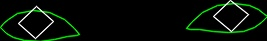
\includegraphics[scale=0.55]{gambar/bab4/30.jpg}
  % Keterangan gambar yang diinputkan
  \caption{Eye Pose Estimation using MediaPipe}
  % Label referensi dari gambar yang diinputkan
  \label{fig:estimasi}
\end{figure}

\subsection{Data Processing}

After the eye pose estimation process is complete, the next step is to group the estimated images into a dataset. This dataset will have 3 different classes, representing the commands to move right, move left, and stop. These classes represent the basic commands to move the wheelchair. 

To improve performance and accuracy, the dataset goes through an optimization process using the Convolutional Neural Network (CNN) algorithm. This step involves customizing and enhancing the CNN model to improve accuracy and efficiency in eye detection. The CNN model used in this research can be seen in Figure \ref{fig:3dlayer}.

%Gambar 3.1
\begin{figure} [ht] \centering
  % Nama dari file gambar yang diinputkan
  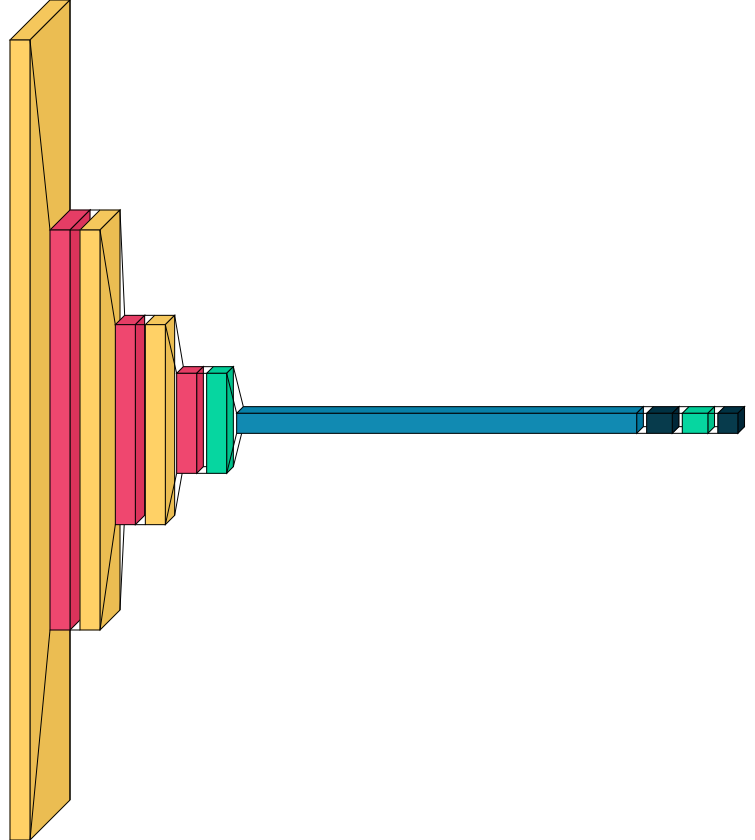
\includegraphics[height=3cm ,width=7cm]{gambar/bab3/3dlayer.png}
  % Keterangan gambar yang diinputkan
  \caption{CNN 3-Dimensional Layer}
  % Label referensi dari gambar yang diinputkan
  \label{fig:3dlayer}
\end{figure}

Before the dataset is trained using a CNN, several preprocessing techniques such as data augmentation and parameter tuning are performed. CNN, several preprocessing techniques are performed such as data augmentation and parameter tuning. Data augmentation is performed to increase the variety of training data and prevent overfitting. The augmentation techniques used include rotation, shearing, and brightness. In addition to augmentation, parameter tuning is also an important part of this process. Parameter tuning involves setting the model's hyperparameters such as the number of convolution layers, filter size, pooling kernel size, dropout rate, and batch size. Also added are some callbacks namely rlrop and early stop. This process aims to find the optimal combination of parameters so that the model can be trained efficiently and accurately.

\subsection{Implementation to NUC}

The implementation of the eye pose detection system onto the Intel NUC begins by installing the necessary software libraries, such as Python, OpenCV, and Mediapipe, onto the device. The trained model is then integrated with the wheelchair control program, connecting the inputs from the camera to the output signals for the wheelchair motors. The Intel NUC is connected to the camera via a USB port and communicates with the wheelchair motor via a serial protocol. The system is optimized to achieve a balance between speed and accuracy, with model and communication parameter settings enabling accurate and responsive eye pose-based wheelchair control.

\subsection{Hardware Block Diagram}

In Figure \ref{fig:aluralat}, it is shown that the camera will take an image of the user's eye. The image will then be processed by Intel NUC using a pre-trained CNN model. The result of the process will generate a pose command that will be sent to the wheelchair motor via Wi-Fi protocol. The wheelchair motor will receive the command and move the wheelchair according to the given command.

%Gambar 3.2
\begin{figure} [ht] \centering
  % Nama dari file gambar yang diinputkan
  \includegraphics[scale=0.55]{gambar/paper5.png}
  % Keterangan gambar yang diinputkan
  \caption{Hardware Block Diagram}
  % Label referensi dari gambar yang diinputkan
  \label{fig:aluralat}
\end{figure}